\documentclass{article}
\usepackage[utf8]{inputenc}
\usepackage[icelandic]{babel}
\usepackage[T1]{fontenc}
\usepackage{graphicx}
\usepackage{mathtools}
\usepackage{amsmath}
\usepackage{amssymb}
\usepackage{minted}


\graphicspath{ {./imgs} }
\title{Blackjack - Viðmótsforritun}
\author{ttb3@hi.is}
\date{\today}


\begin{document}
\maketitle


\section*{Hönnun}
Fyrsta (og eina) hönnunin var gerð með blað og penna lokaútkoman fór ekki alveg eftir henni en var á svipuðum nótum.
\begin{center}
    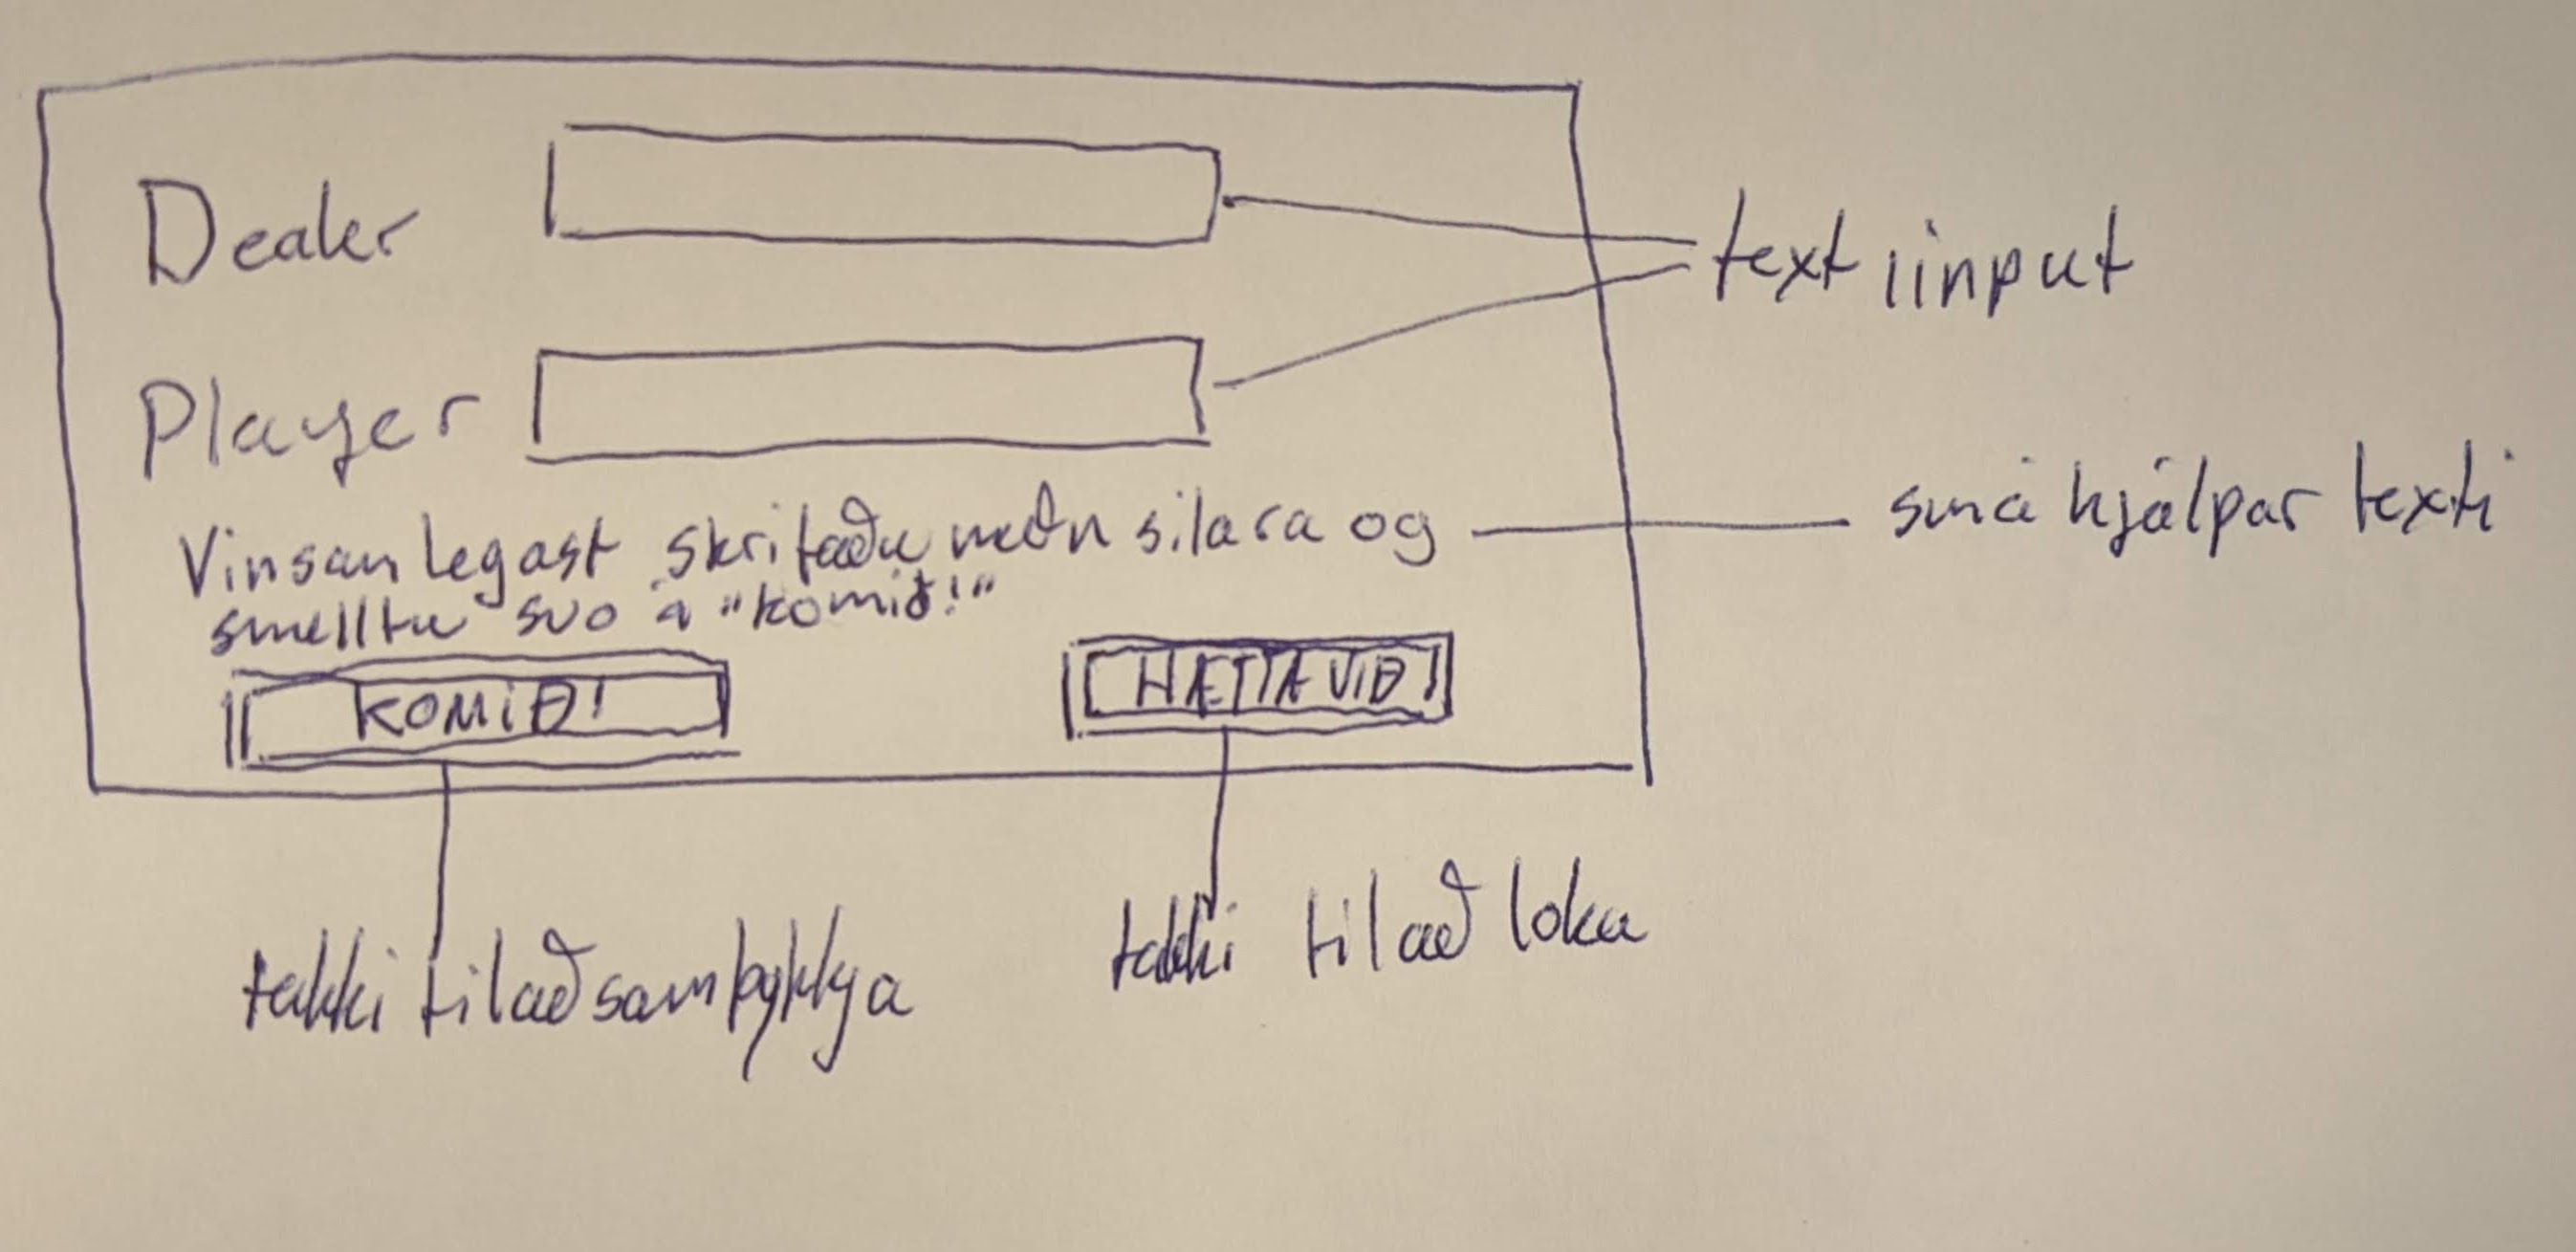
\includegraphics[scale=0.12]{sketch1.jpg}
\end{center}
byrjaði að hanna dialogið en útfærði það samt síðast, það hjálpaði því undir lokin ég kominn með betra grip á fxml-inu og náði að útfæra útlitið nær hönnuninni en í útlinu fyrir leikinn sjálfann.
\newpage
\begin{center}
    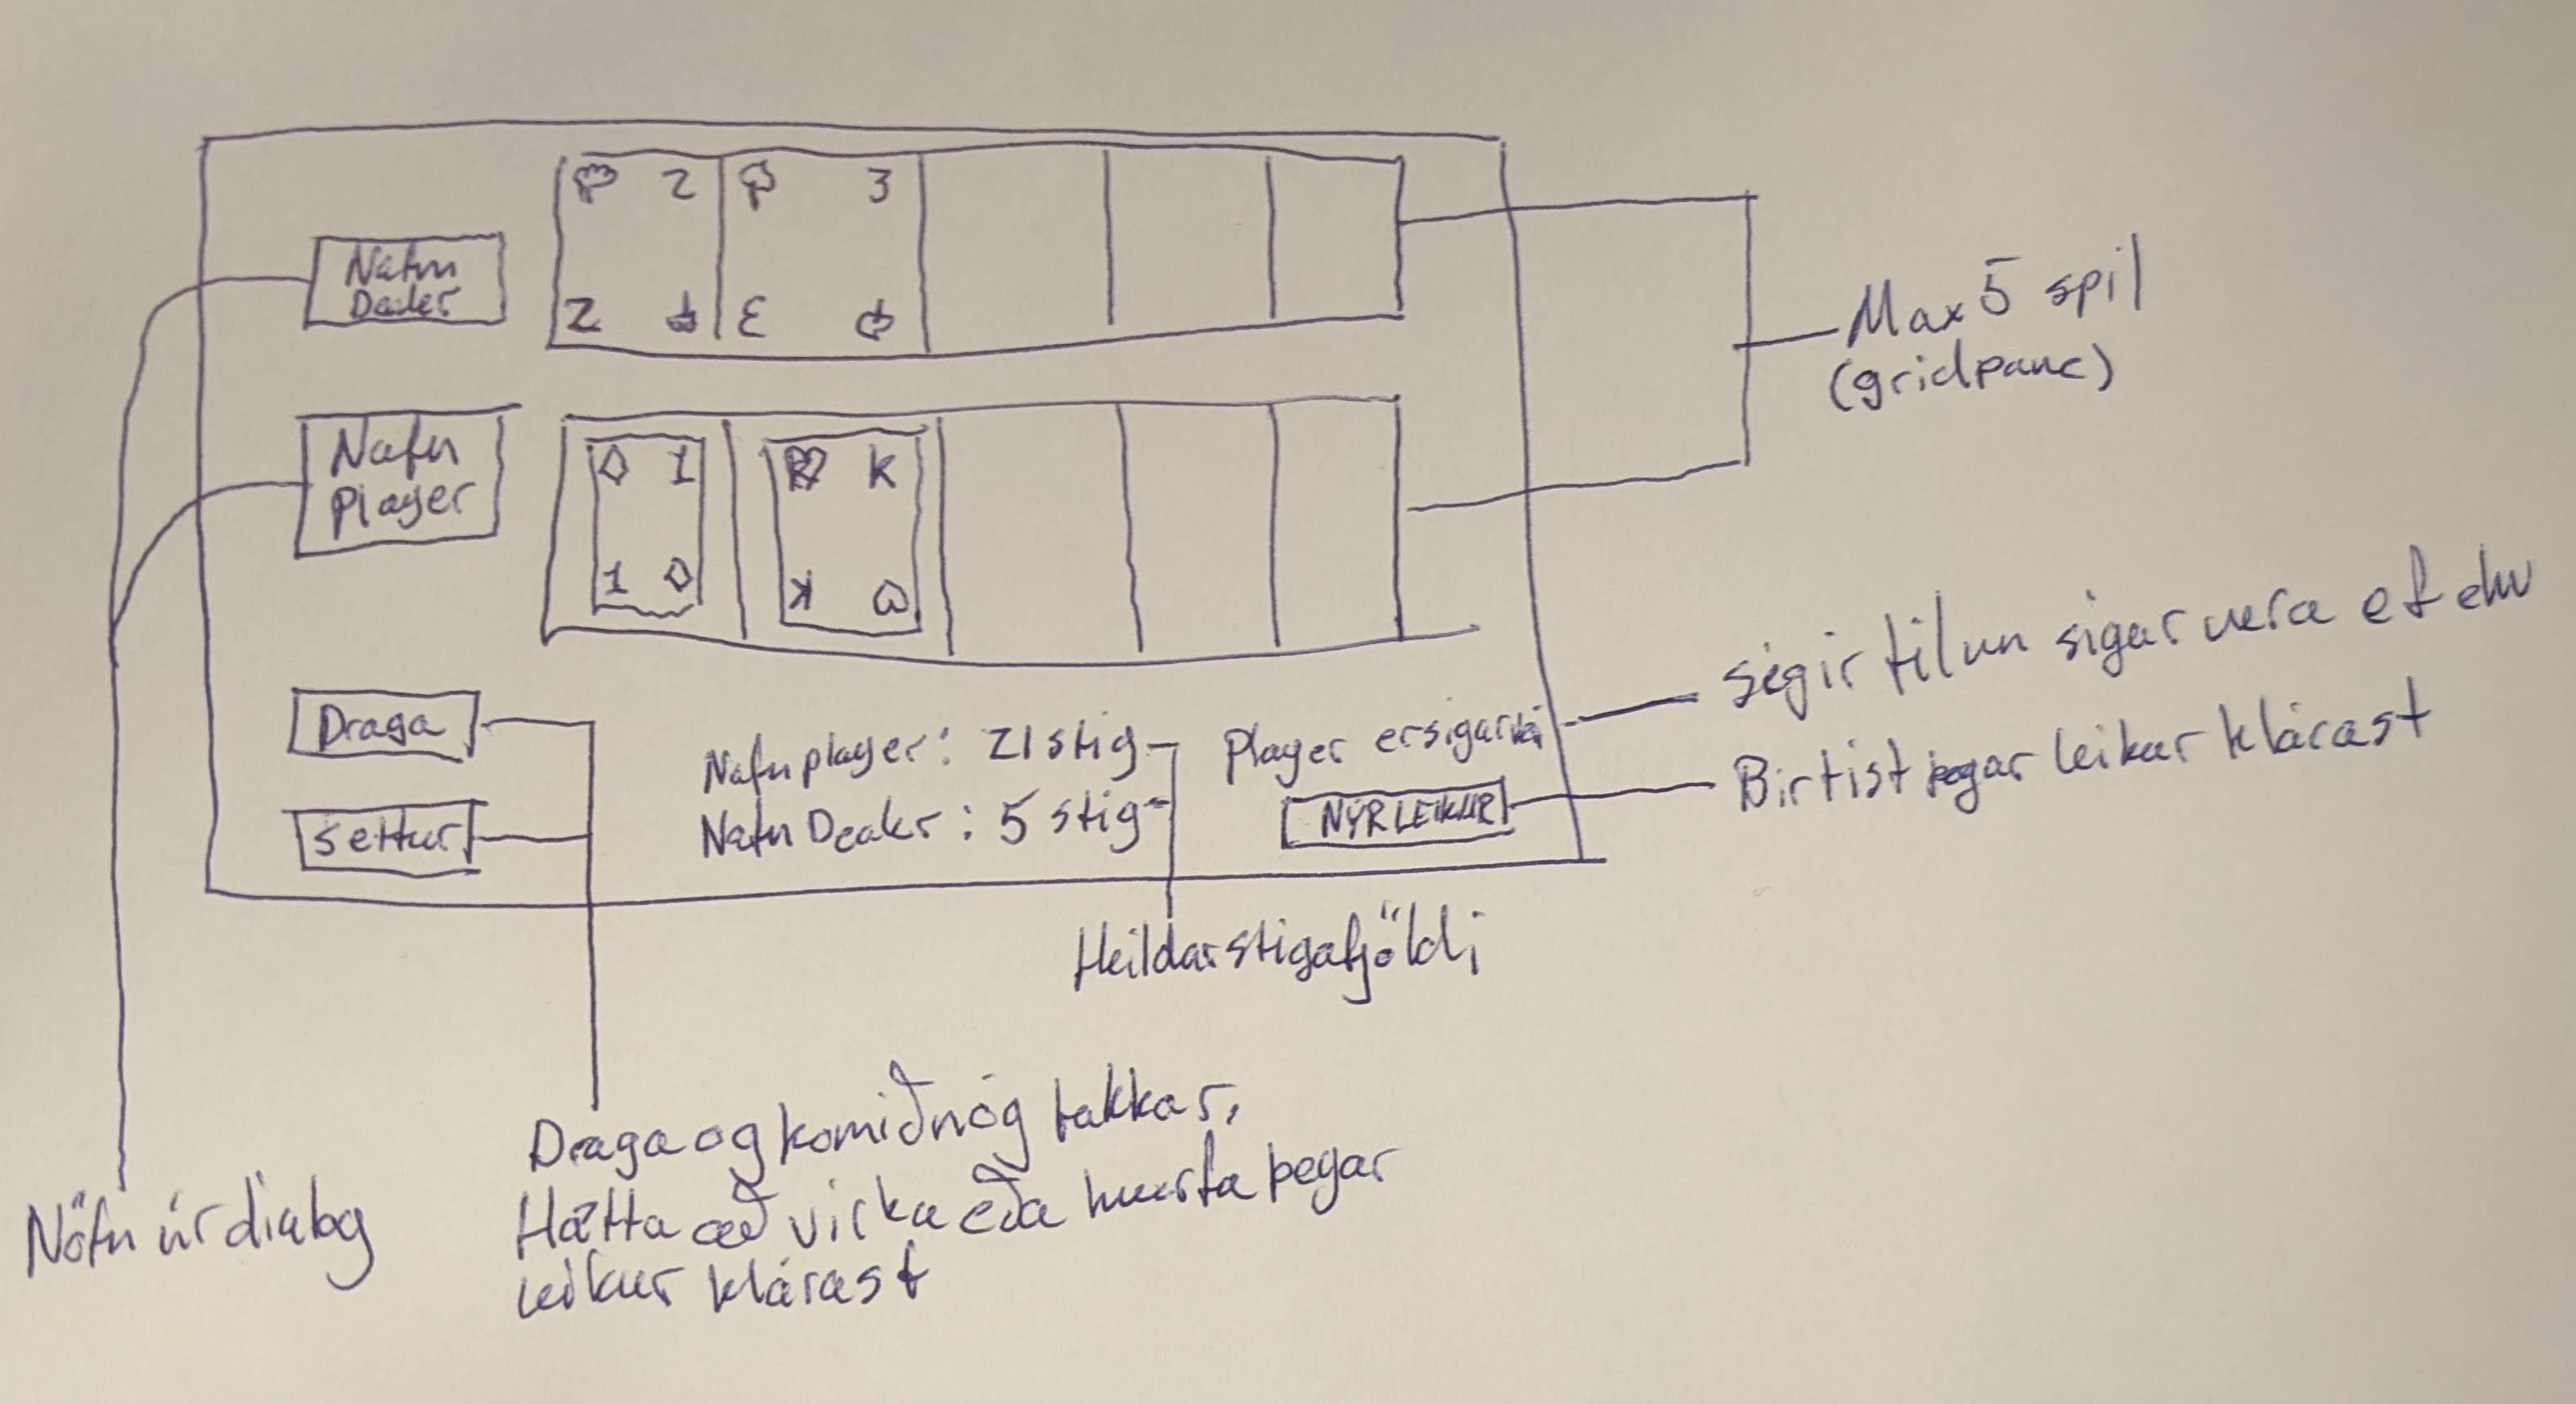
\includegraphics[scale=0.1]{sketch2.jpg}
\end{center}
Hönnunin fyrir leikinn sjálfann var aðeins djarfari og mér tókst verr að fylgja hönnuninni í því en dialoginu. útlitið hélst samt mestmegnis eins þrátt fyrir smávæginlegar breytingar á röðun hlutanna.
Meginatriði hönnunar sem ég var að miða á voru  nokkur. 
\begin{enumerate}
    \item Fyrst að hafa sýnileikann góðann, þetta tókst vel þar sem í raun allt nema spilin sjálf er bara svartur texti á hvítum bakgrunn.
    \item Samræmi var einfalt vegna þess að Scenebuilder virkar ekki hjá mér og gerir mér því erfitt að flækja hönnunina mikið, þ.e. allt lýtur frekar eins út.
    \item Kunnugleiki, takkarnir bjóða ekki upp á mikið val, ef þú hefur notað takka áður veistu hvað er að fara gerast.
    \item Stýring er auðveld, meira að segja fyrir þá sem kunna ekki spilið þar sem tölvan sér um alla stóra útreikninga, plús ef maður er að spila sem bankinn, þarf maður ekki einu sinni að gera neitt.
    \item Endurgjöfin hefði mátt vera aðeins meira áberandi, stærra letur eða bold eða ehv álíka, en hún virkar nógu vel.
    \item Takmörkun er mikil þar sem það eru bara 3 takkar sem hægt er að ýta á eftir að leikur er byrjaður, draga, komið nóg og nýr leikur. Enginn af þeim getur brotið kerfið.
\end{enumerate}

\newpage
\section*{Keyrsla}
þegar forritið er fyrst keyrt birtist dialog sem biður um nöfn spilara, annar er 'banki' eða 'dealer' og gerir tölvan fyrir hann sjálf útfrá stöðu leiksins, hinn spilarinn er 'player' og fær að ráða hvenær hann er kominn með nóg af spilum og hvenær hann vill draga.
það er aðeins hægt að byrja leik þegar báðir leikmenn eru komnir með nafn, eins og sést á mynd 2 er takkinn ennþá grár þegar það er bara komið eitt nafn en svo á mynd 3 verður takkinn blár og "smellanlegur" 
\begin{center}
    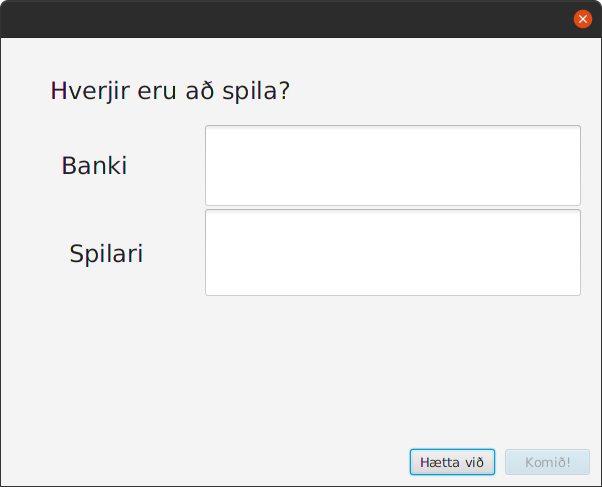
\includegraphics[scale=0.27]{dialog.png}
    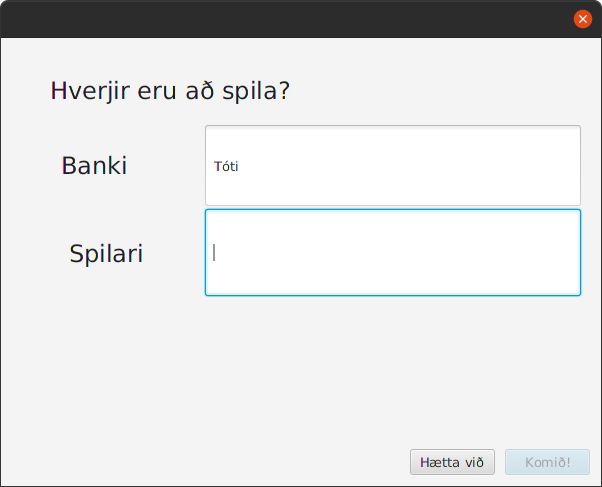
\includegraphics[scale=0.27]{dialog2.png}
    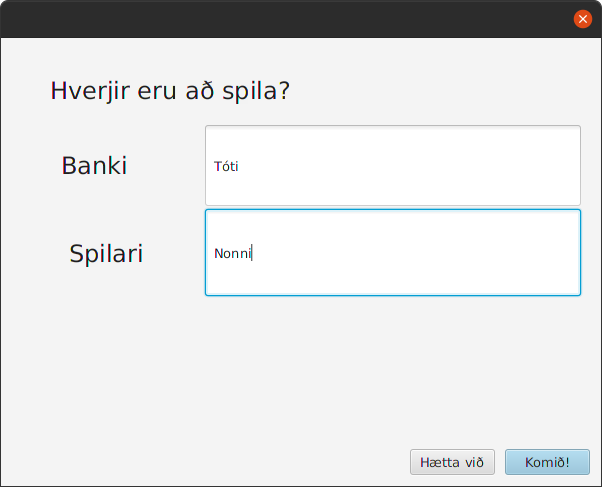
\includegraphics[scale=0.27]{Dialog3.png}
\end{center}

eftir að nöfnin eru gefin er birtur annar skjár með leiknum sjálfum. Þar gefst spilurum einn kostur, að byrja leik.
Þegar leikur er byrjaður er 'player' sá eini sem getur haft áhrif á leikinn, hann getur dregið spil eða sagst vera góðum með núverandi hendi. 
Í bakgrunninum er athugað hvort annar spilaranna sé yfir 21 og ef svo er þá vinnur hinn. Það eru fleiri athugannir gerðar, en þessi er mest áberandi.
\begin{center}
    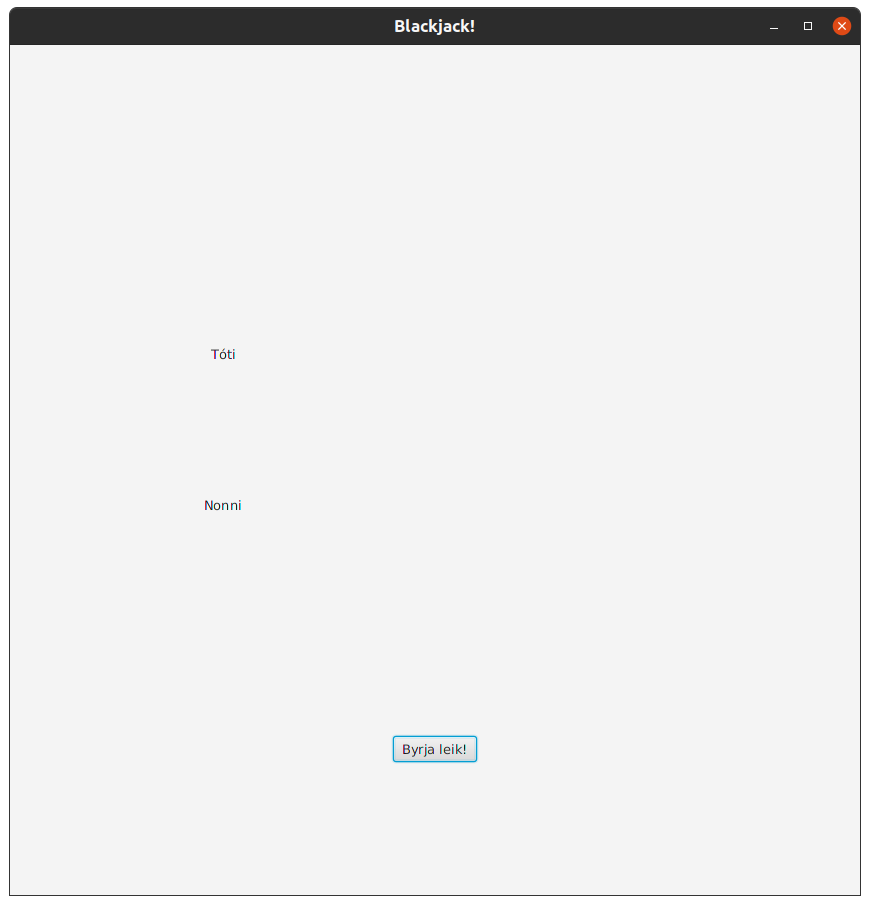
\includegraphics[scale=0.17]{bj1.png}
    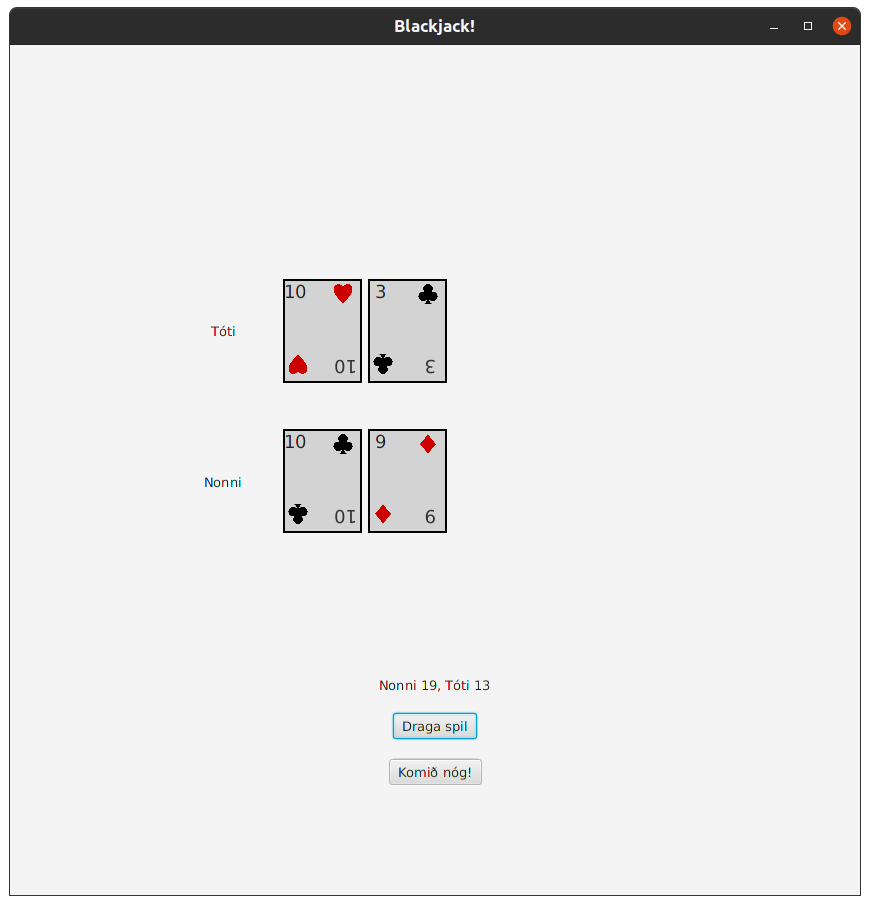
\includegraphics[scale=0.17]{bj2.png}
    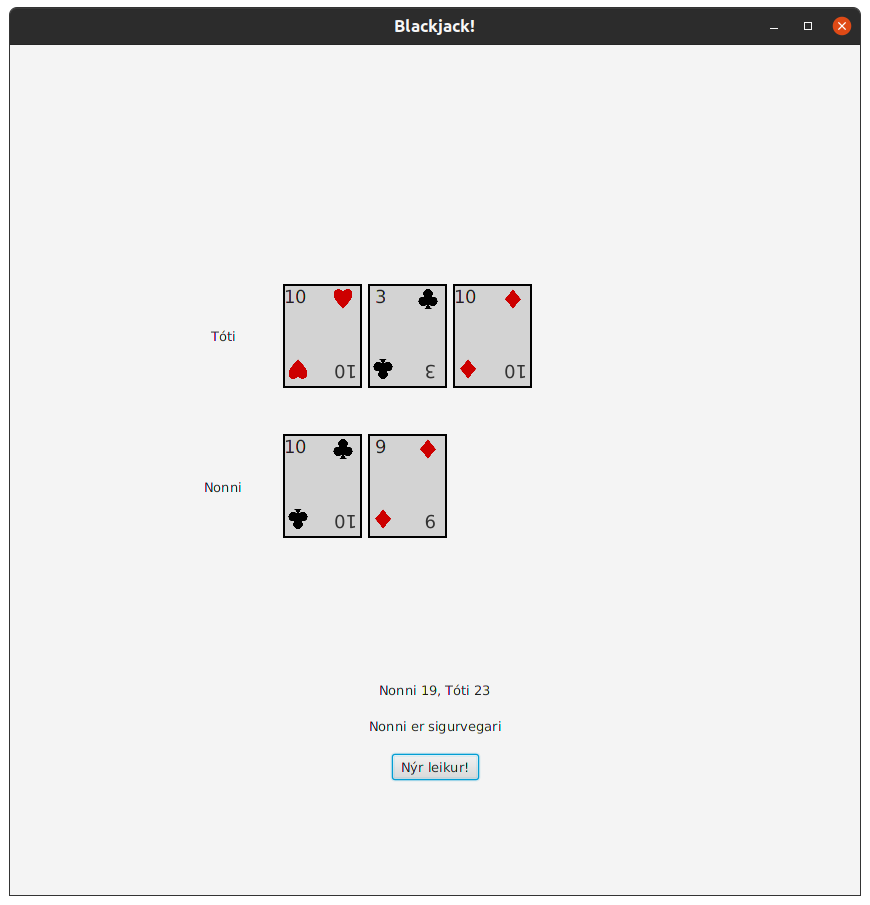
\includegraphics[scale=0.17]{bj3.png}
    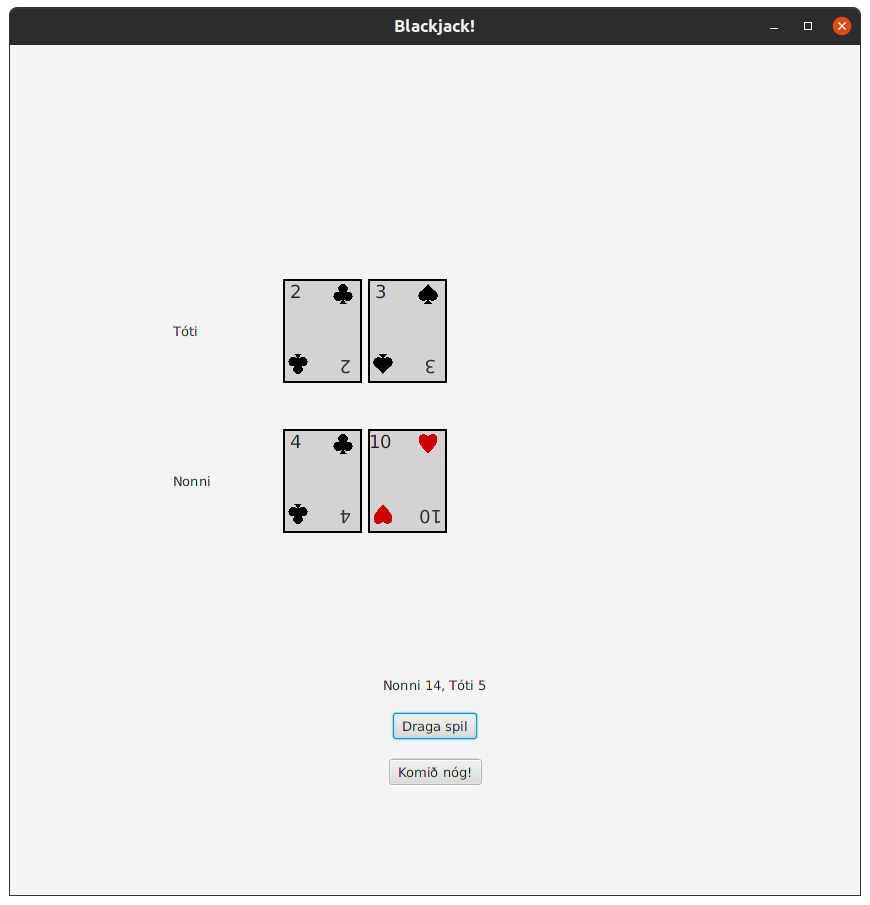
\includegraphics[scale=0.17]{bj4.png}
    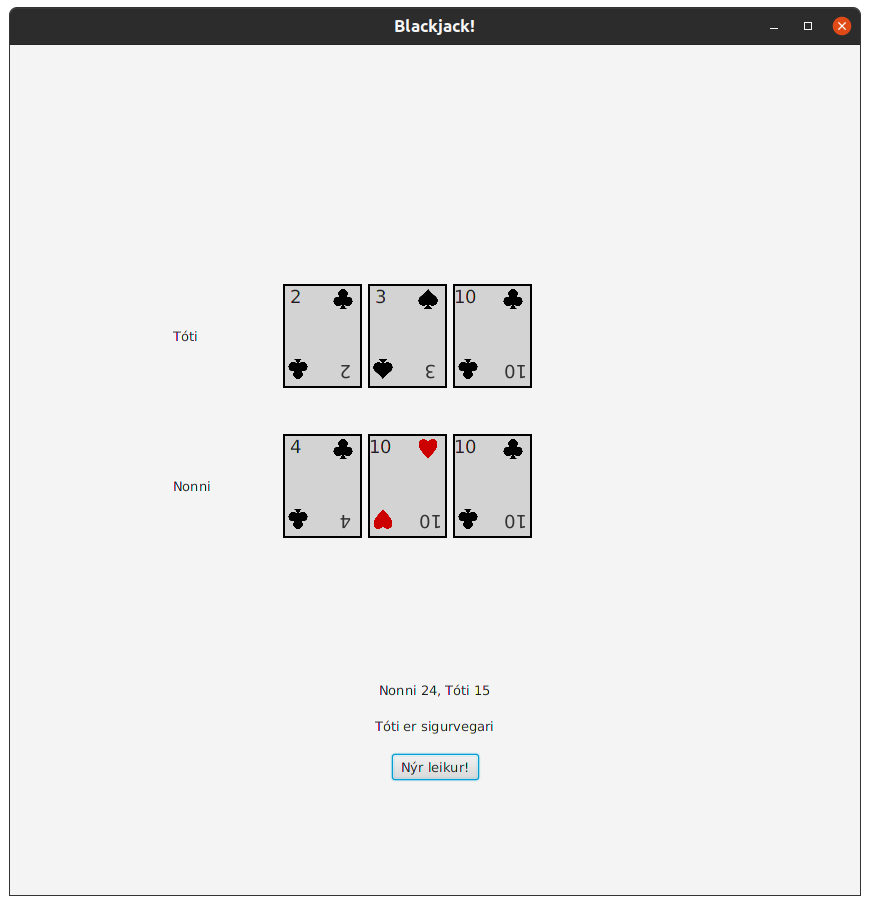
\includegraphics[scale=0.17]{bj6.png}
\end{center}

\end{document}